\documentclass{vkr}
\usepackage{enumitem}
\renewcommand{\labelitemi}{\textbullet}
\usepackage[english, russian]{babel} % переносы
\usepackage{graphicx} % для вставки картинок
\graphicspath{{images/}} % путь к изображениям
\usepackage[hidelinks]{hyperref}
\usepackage{float} % определяет метод H для рисунка с переносом на следующую страницу, ели не помещается
\usepackage{pdflscape}
\addto{\captionsrussian}{\renewcommand{\refname}{СПИСОК ИСПОЛЬЗОВАННЫХ ИСТОЧНИКОВ}}
\usepackage{xltabular} % для вставки таблиц
\usepackage{makecell}
\renewcommand\theadfont{} % шрифт в /thead
\usepackage{array} % для определения новых типов столбцов таблиц
\newcolumntype{T}{>{\centering\arraybackslash}X} % новый тип столбца T - автоматическая ширина столбца с выравниванием по центру
\newcolumntype{R}{>{\raggedleft\arraybackslash}X} % новый тип столбца R - автоматическая ширина столбца с выравниванием по правому краю
\newcolumntype{C}[1]{>{\centering\let\newline\\\arraybackslash\hspace{0pt}}m{#1}} % новый тип столбца C - фиксированная ширина столбца с выравниванием по центру
\newcolumntype{r}[1]{>{\raggedleft\arraybackslash}p{#1}} % новый тип столбца r - фиксированная ширина столбца с выравниванием по правому краю
\newcommand{\centrow}{\centering\arraybackslash} % командой \centrow можно центрировать одну ячейку (заголовок) в столбце типа X или p, оставив в оcтальных ячейках другой тип выравнивания
\newcommand{\finishhead}{\endhead\hline\endlastfoot}
\newcommand{\continuecaption}[1]{\captionsetup{labelformat=empty} \caption[]{#1}\\ \hline }
\usepackage{etoolbox}
\AtBeginEnvironment{xltabular}{\refstepcounter{tablecnt}} % подсчет таблиц xltabular, обычные таблицы подсчитываются в классе

\usepackage[tableposition=top]{caption} % подпись таблицы вверху
\captionsetup{strut=off}
\setlength{\intextsep}{0pt} % Vertical space above & below [h] floats
\setlength{\textfloatsep}{0pt} % Vertical space below (above) [t] ([b]) floats
\DeclareCaptionLabelFormat{gostfigure}{Рисунок #2} %подпись рисунка
\DeclareCaptionLabelFormat{gosttable}{Таблица #2} %подпись таблицы
\DeclareCaptionLabelSeparator{gost}{~--~} %разделитель в рисунках и таблицах
\captionsetup{labelsep=gost}
\captionsetup[figure]{aboveskip=10pt,belowskip=4mm,justification=centering,labelformat=gostfigure} % настройка подписи рисунка
\captionsetup[table]{font={stretch=1.41},skip=0pt,belowskip=0pt,aboveskip=8.5pt,singlelinecheck=off,labelformat=gosttable} % настройка подписи таблицы

\setlength{\LTpre}{8mm} % отступ сверху таблицы
\setlength{\LTpost}{6mm} % отступ снизу таблицы

\usepackage{enumitem}
\setlist{nolistsep,wide=\parindent,itemindent=*} % отступы вокруг списков, выравнивание с учетом разделителя

\usepackage{color} %% это для отображения цвета в коде
\usepackage{listings} %% листинги кода
\setmonofont[Scale=0.7]{Verdana} % моноширный шрифт для листинга

\definecolor{codegreen}{rgb}{0,0.6,0}
\definecolor{codegray}{rgb}{0.5,0.5,0.5}
\definecolor{codepurple}{rgb}{0.58,0,0.82}

\lstset{ %
language=C,                 % выбор языка для подсветки (здесь это С)
numbers=left,               % где поставить нумерацию строк (слева\справа)
numberstyle=\tiny,           % размер шрифта для номеров строк
stepnumber=1,                   % размер шага между двумя номерами строк
numbersep=5pt,                % как далеко отстоят номера строк от подсвечиваемого кода
commentstyle=\color{codegreen},
keywordstyle=\color{magenta},
numberstyle=\tiny\color{codegray},
stringstyle=\color{codepurple},
basicstyle=\linespread{0.95}\ttfamily,
backgroundcolor=\color{white}, % цвет фона подсветки - используем \usepackage{color}
showspaces=false,            % показывать или нет пробелы специальными отступами
showstringspaces=false,      % показывать или нет пробелы в строках
showtabs=false,             % показывать или нет табуляцию в строках
frame=single,              % рисовать рамку вокруг кода
tabsize=2,                 % размер табуляции по умолчанию равен 2 пробелам
captionpos=t,              % позиция заголовка вверху [t] или внизу [b] 
breaklines=true,           % автоматически переносить строки (да\нет)
breakatwhitespace=false, % переносить строки только если есть пробел
escapeinside={\%*}{*)}   % если нужно добавить комментарии в коде
}

\makeatletter % чтобы допускались русские комментарии в листингах
\lst@InputCatcodes
\def\lst@DefEC{%
 \lst@CCECUse \lst@ProcessLetter
  ^^80^^81^^82^^83^^84^^85^^86^^87^^88^^89^^8a^^8b^^8c^^8d^^8e^^8f%
  ^^90^^91^^92^^93^^94^^95^^96^^97^^98^^99^^9a^^9b^^9c^^9d^^9e^^9f%
  ^^a0^^a1^^a2^^a3^^a4^^a5^^a6^^a7^^a8^^a9^^aa^^ab^^ac^^ad^^ae^^af%
  ^^b0^^b1^^b2^^b3^^b4^^b5^^b6^^b7^^b8^^b9^^ba^^bb^^bc^^bd^^be^^bf%
  ^^c0^^c1^^c2^^c3^^c4^^c5^^c6^^c7^^c8^^c9^^ca^^cb^^cc^^cd^^ce^^cf%
  ^^d0^^d1^^d2^^d3^^d4^^d5^^d6^^d7^^d8^^d9^^da^^db^^dc^^dd^^de^^df%
  ^^e0^^e1^^e2^^e3^^e4^^e5^^e6^^e7^^e8^^e9^^ea^^eb^^ec^^ed^^ee^^ef%
  ^^f0^^f1^^f2^^f3^^f4^^f5^^f6^^f7^^f8^^f9^^fa^^fb^^fc^^fd^^fe^^ff%
  ^^^^20ac^^^^0153^^^^0152%
  % Basic Cyrillic alphabet coverage
  ^^^^0410^^^^0411^^^^0412^^^^0413^^^^0414^^^^0415^^^^0416^^^^0417%
  ^^^^0418^^^^0419^^^^041a^^^^041b^^^^041c^^^^041d^^^^041e^^^^041f%
  ^^^^0420^^^^0421^^^^0422^^^^0423^^^^0424^^^^0425^^^^0426^^^^0427%
  ^^^^0428^^^^0429^^^^042a^^^^042b^^^^042c^^^^042d^^^^042e^^^^042f%
  ^^^^0430^^^^0431^^^^0432^^^^0433^^^^0434^^^^0435^^^^0436^^^^0437%
  ^^^^0438^^^^0439^^^^043a^^^^043b^^^^043c^^^^043d^^^^043e^^^^043f%
  ^^^^0440^^^^0441^^^^0442^^^^0443^^^^0444^^^^0445^^^^0446^^^^0447%
  ^^^^0448^^^^0449^^^^044a^^^^044b^^^^044c^^^^044d^^^^044e^^^^044f%
  ^^^^0401^^^^0451%
  %%%
  ^^00}
\lst@RestoreCatcodes
\makeatother


% Режим шаблона (должен быть включен один из трех)
%\ВКРtrue
\Практикаtrue
%\Курсоваяtrue

\newcommand{\Дисциплина}{<<Проектирование и архитектура программных систем>>} % для курсовой
\newcommand{\КодСпециальности}{09.03.04} % Курсовая
\newcommand{\Специальность}{Программная инженерия} % Курсовая
\newcommand{\Тема}{Разработка web-сайта «Русатом – Аддитивные технологии» на платформе} % ВКР Курсовая
\newcommand{\ТемаВтораяСтрока}{1С-Битрикс}
\newcommand{\ГдеПроводитсяПрактика}{ООО «Предприятие ВТИ-Сервис»} % для практики
\newcommand{\РуководительПрактПредпр}{Федосов Д. В.} % для практики
\newcommand{\ДолжнРуководительПрактПредпр}{директор} % для практики
\newcommand{\РуководительПрактУнивер}{Чаплыгин А. А.} % для практики
\newcommand{\ДолжнРуководительПрактУнивер}{к.т.н. доцент} % для практики
\newcommand{\Автор}{И. И. Иванов}
\newcommand{\АвторРод}{Иванова И.И.}
\newcommand{\АвторПолностьюРод}{Тарасова Артема Вячеславовича} % для практики
\newcommand{\Шифр}{хх-хх-хххх}
\newcommand{\Курс}{4 } % для практики
\newcommand{\Группа}{ПО-11б}
\newcommand{\Руководитель}{А. А. Чаплыгин} % для ВКР и курсовой
\newcommand{\Нормоконтроль}{А. А. Чаплыгин} % для ВКР
\newcommand{\ЗавКаф}{А. В. Малышев} % для ВКР
\newcommand{\ДатаПриказа}{«07» апреля 2023~г.} % для ВКР
\newcommand{\НомерПриказа}{1505-с} % для ВКР
\newcommand{\СрокПредоставления}{«13» июня 2023~г.} % для ВКР, курсового

\begin{document}
\maketitle
\ifПрактика{}\else{
   \newpage
\begin{center}
\large\textbf{Минобрнауки России}

\large\textbf{Юго-Западный государственный университет}
\vskip 1em
\normalsize{Кафедра программной инженерии}
\vskip 1em
\ifВКР{
        \begin{flushright}
        \begin{tabular}{p{.4\textwidth}}
        \centrow УТВЕРЖДАЮ: \\
        \centrow Заведующий кафедрой \\
        \hrulefill \\
        \setarstrut{\footnotesize}
        \centrow\footnotesize{(подпись, инициалы, фамилия)}\\
        \restorearstrut
        «\underline{\hspace{1cm}}»
        \underline{\hspace{3cm}}
        20\underline{\hspace{1cm}} г.\\
        \end{tabular}
        \end{flushright}
        }\fi
\end{center}
\vspace{1em}
  \begin{center}
  \large
\ifВКР{
ЗАДАНИЕ НА ВЫПУСКНУЮ КВАЛИФИКАЦИОННУЮ РАБОТУ
  ПО ПРОГРАММЕ БАКАЛАВРИАТА}
  \else
ЗАДАНИЕ НА КУРСОВУЮ РАБОТУ (ПРОЕКТ)
\fi
\normalsize
  \end{center}
\vspace{1em}
{\parindent0pt
  Студента \АвторРод, шифр\ \Шифр, группа \Группа
  
1. Тема «\Тема\ \ТемаВтораяСтрока»
\ifВКР{
утверждена приказом ректора ЮЗГУ от \ДатаПриказа\ № \НомерПриказа
}\fi.

2. Срок предоставления работы к защите \СрокПредоставления

3. Исходные данные для создания программной системы:

3.1. Перечень решаемых задач:}

\renewcommand\labelenumi{\theenumi)}

\begin{enumerate}
\item проанализировать IT-инфраструктуру предприятия;
\item  разработать концептуальную модель системы управления IT-ин\-фра\-струк\-турой предприятия на основе подхода к управлению и организации ИТ-услуг ITSM;
\item спроектировать программную систему управления IT-ин\-фра\-струк\-турой предприятия;
\item сконструировать и протестировать программную систему управления IT-инфраструктурой предприятия.
\end{enumerate}

{\parindent0pt
  3.2. Входные данные и требуемые результаты для программы:}

\begin{enumerate}
\item Входными данными для программной системы являются: данные
справочников комплектующих, конфигураций, ПО, критериев качества SLA,
ИТ-услуг, департаментов компании; технические данные ИТ-ресурсов; данные входящих заявок на ИТ-ресурсы; данные запросов поставщикам на комплектующие.
\item Выходными данными для программной системы являются: сформированные заявки на обслуживание ИТ-ресурсов; сформированные запросы на
закупку комплектующих; сведения о выполненных работах по заявкам; статусы заявок; выходные отчеты (инфографика) – по качеству услуг, по состоянию ИТ-ресурсов, по деятельности ИТ-отдела, по стоимости обслуживания
ИТ-ресурсов, воронка заявок.
\end{enumerate}

{\parindent0pt

  4. Содержание работы (по разделам):
  
  4.1. Введение.
  
  4.1. Анализ предметной области.
  
4.2. Техническое задание: основание для разработки, назначение разработки,
требования к программной системе, требования к оформлению документации.

4.3. Технический проект: общие сведения о программной системе, проект
данных программной системы, проектирование архитектуры программной системы, проектирование пользовательского интерфейса программной системы.

4.4. Рабочий проект: спецификация компонентов и классов программной системы, тестирование программной системы, сборка компонентов программной системы.

4.5. Заключение.

4.6. Список использованных источников.

5. Перечень графического материала:

\списокПлакатов

\vskip 2em
\begin{tabular}{p{6.8cm}C{3.8cm}C{4.8cm}}
Руководитель \ifВКР{ВКР}\else работы (проекта) \fi & \lhrulefill{\fill} & \fillcenter\Руководитель\\
\setarstrut{\footnotesize}
& \footnotesize{(подпись, дата)} & \footnotesize{(инициалы, фамилия)}\\
\restorearstrut
Задание принял к исполнению & \lhrulefill{\fill} & \fillcenter\Автор\\
\setarstrut{\footnotesize}
& \footnotesize{(подпись, дата)} & \footnotesize{(инициалы, фамилия)}\\
\restorearstrut
\end{tabular}
}

\renewcommand\labelenumi{\theenumi.}

   \abstract{РЕФЕРАТ}

Объем работы равен \formbytotal{lastpage}{страниц}{е}{ам}{ам}. Работа содержит \formbytotal{figurecnt}{иллюстраци}{ю}{и}{й}, \formbytotal{tablecnt}{таблиц}{у}{ы}{}, \arabic{bibcount} библиографических источников и \formbytotal{числоПлакатов}{лист}{}{а}{ов} графического материала. Количество приложений – 2. Графический материал представлен в приложении А. Фрагменты исходного кода представлены в приложении Б.

Перечень ключевых слов: коммерческий сайт, Система, CMS, Битрикс, Joomla, аддитивные технологии, 3D-принтеры, услуги, сервисы, информатизация, автоматизация, информационные технологии, веб-форма,  Apache, классы, база данных, средства защиты информации, подсистема, компонент, модуль, сущность, информационный блок, метод, контент-редактор, администратор, пользователь, web-сайт.

Объектом разработки является web-сайт компании,  занимающейся производством 3D-принтеров, выпуском оборудования для создания порошков, разработкой программного обеспечения и организацией центров аддитивного производства.

Целью выпускной квалификационной работы является привлечение клиентов, увеличение заказов, информирование о продукции и услугах путем создания сайта компании.

В процессе создания сайта были выделены основные сущности путем создания информационных блоков, использованы классы и методы модулей, обеспечивающие работу с сущностями предметной области, а также корректную работу web-сайта, разработаны разделы, содержащие информацию о компании, ее деятельности, производимой продукции и услугах, разработан сервис по заказу 3D-деталей.

При разработке сайта использовалась система управления контентом "<1С-Битрикс: Управление сайтом">.

Разработанный сайт был успешно внедрен в компании.

\selectlanguage{english}
\abstract{ABSTRACT}
  
The volume of work is \formbytotal{lastpage}{page}{}{s}{s}. The work contains \formbytotal{figurecnt}{illustration}{}{s}{s}, \formbytotal{tablecnt}{table}{}{s}{s}, \arabic{bibcount} bibliographic sources and \formbytotal{числоПлакатов}{sheet}{}{s}{s} of graphic material. The number of applications is 2. The graphic material is presented in annex A. The layout of the site, including the connection of components, is presented in annex B.

List of keywords: commercial website, System, CMS, Bitrix, Joomla, additive technologies, 3D printers, services, services, informatization, automation, information technology, web form, Apache, classes, database, component, module, entity, information block, method, content editor, administrator, user, web site.

The object of the research is the analysis of information technologies for the development of a production company's website.

The object of the development is the website of a company engaged in the production of 3D printers, the production of equipment for the creation of powders, software development and the organization of additive manufacturing centers.

The purpose of the final qualifying work is to attract customers, increase orders, inform about products and services by creating a company website.

In the process of creating the site, the main entities were identified by creating information blocks, classes and methods of modules were used to ensure work with the entities of the subject area, as well as the correct operation of the website, sections containing information about the company, its activities, products and services were developed, a service for ordering 3D parts was developed.

When developing the site, the content management system <<1C – Bitrix: Site Management>> was used.

The developed website was successfully implemented in the company.
\selectlanguage{russian}
}\fi
\tableofcontents
\section*{ОБОЗНАЧЕНИЯ И СОКРАЩЕНИЯ}

БД -- база данных.

ИС -- информационная система.

ИТ -- информационные технологии. 

КТС -- комплекс технических средств.

ОМТС -- отдел материально-технического снабжения. 

ПО -- программное обеспечение.

РП -- рабочий проект.

СУБД -- система управления базами данных.

ТЗ -- техническое задание.

ТП -- технический проект.

UML (Unified Modelling Language) -- язык графического описания для объектного моделирования в области разработки программного обеспечения.

\ifПрактика{}\else{\section*{ВВЕДЕНИЕ}
\addcontentsline{toc}{section}{ВВЕДЕНИЕ}

Аддитивные технологии (АТ) начали активно развиваться со времени получения первых трехмерных изображений изделий на дисплеях компьютеров. Начало положила стереолитография, затем довольно многочисленные новые принципы стали называть технологиями быстрого прототипирования, затем укоренилось название "<Аддитивные технологии">. Интенсивность развития данных технологий не имеет аналогов. АТ изменили процессы проектирования и конструирования изделий, превратив их в процессы непрерывного создания изделий. Современные проектирование и производство изделий невозможно представить без данного рода технологий. 3D-принтеры стали такими же распространенными, как и персональные компьютеры. С помощью 3D-принтеров получают ткани, обувь, продукты питания, а также выращивают человеческие органы. Во многих отраслях, например, в космической отрасли, альтернативы аддитивным технологиям нет.

АТ предполагают изготовление детали методом послойного нанесения материала, в отличие от традиционных методов формирования детали, за счёт удаления материала из массива заготовки.

При использовании АТ все стадии реализации проекта от идеи до материализации находятся в единой технологической цепи, в которой каждая технологическая операция выполняется в цифровой CAD/CAM/CAE-системе.

Современные компании, видя, как развиваются информационные технологии, пытаются использовать их выгодно для своего бизнеса, поэтому запускают свой web-сайт. С его помощью предприятие может заявить о себе, проинформировать потенциального заказчика об услугах или продуктах, которые предоставляет, а также позволяет пользователям сделать с помощью сайта онлайн-заказ, произвести покупку или оплатить счета.

Сайт считается лицом компании и может существенно повысить ее имидж. Любой пользователь сети Интернет сможет получить необходимую информацию о компании в любой момент, появляется возможность найти контактные телефоны, адрес и e-mail, чтобы связаться с компанией. Сейчас большинство клиентов узнают о ее существовании именно через сайт. Поэтому сайт можно назвать самой лучшей рекламой. 

Главной задачей профессионально построенного сайта является превращение посетителя, зашедшего на сайт, в потенциального клиента.

\emph{Цель настоящей работы} – разработка web-сайта компании для привлечения новой аудитории, увеличения заказов, рекламы продукции и услуг компании. Для достижения поставленной цели необходимо решить \emph{следующие задачи:}
\begin{itemize}
\item провести анализ предметной области;
\item разработать концептуальную модель web-сайта;
\item спроектировать web-сайт;
\item реализовать сайт средствами web-технологий.
\end{itemize}

\emph{Структура и объем работы.} Отчет состоит из введения, 4 разделов основной части, заключения, списка использованных источников, 2 приложений. Текст выпускной квалификационной работы равен \formbytotal{lastpage}{страниц}{е}{ам}{ам}.

\emph{Во введении} сформулирована цель работы, поставлены задачи разработки, описана структура работы, приведено краткое содержание каждого из разделов.

\emph{В первом разделе} на стадии описания технической характеристики предметной области приводится сбор информации о деятельности компании, для которой осуществляется разработка сайта.

\emph{Во втором разделе} на стадии технического задания приводятся требования к разрабатываемому сайту.

\emph{В третьем разделе} на стадии технического проектирования представлены проектные решения для web-сайта.

\emph{В четвертом разделе} приводится список классов и их методов, использованных при разработке сайта, производится тестирование разработанного сайта.

В заключении излагаются основные результаты работы, полученные в ходе разработки.

В приложении А представлен графический материал.
В приложении Б представлены фрагменты исходного кода. 
}\fi
\section{Анализ предметной области}
\subsection{Принципы работы web-платформы для поиска работы}

Web-платформа для поиска работы — это программно-информационная система, предназначенная для автоматизации процессов взаимодействия между соискателями и работодателями. Она позволяет пользователям эффективно находить друг друга, обмениваться информацией и заключать трудовые соглашения. Основная цель платформы — упрощение поиска работы для соискателей и подбора персонала для работодателей, минимизируя временные и ресурсные затраты.

\subsubsection{Регистрация и управление пользователями}

Для использования платформы пользователи проходят процесс регистрации. Соискатели создают профиль, указывая личные данные, а также информацию о профессиональном опыте, образовании и навыках. Работодатели регистрируются как представители компании, указывая данные о компании и контактные данные. После регистрации пользователи получают доступ к личному кабинету, где могут управлять своими данными, резюме или вакансиями. Платформа обеспечивает безопасность данных пользователей, используя шифрование и механизмы авторизации, а также соответствует требованиям законодательства о защите персональных данных.

\subsubsection{Создание и публикация резюме}

Соискатели могут создавать резюме, указывая профессиональные навыки, опыт работы, образование, желаемую зарплату, тип занятости и другие параметры. Платформа предоставляет шаблоны резюме для упрощения процесса заполнения. После создания резюме проходит модерацию, чтобы исключить некорректные или мошеннические записи. Опубликованные резюме становятся доступны для просмотра работодателями, которые могут фильтровать их по заданным критериям.

\subsubsection{Создание и публикация вакансий}

Работодатели могут публиковать вакансии, указывая требования к кандидатам, условия работы, а также описание компании и контактные данные. Как и резюме, вакансии проходят модерацию, чтобы обеспечить их соответствие правилам платформы и законодательству. Опубликованные вакансии становятся доступны для соискателей, которые могут искать их с помощью фильтров.

\subsubsection{Поиск и отклики}

Платформа предоставляет функционал поиска, который позволяет соискателям находить подходящие вакансии, а работодателям — подходящих кандидатов. Соискатели могут использовать фильтры и ключевые слова для поиска вакансий, а затем отправлять отклики, прикрепляя своё резюме. Работодатели, в свою очередь, могут искать резюме по аналогичным критериям и отправлять приглашения на собеседование.

\subsection{Преимущества и недостатки web-платформ для поиска работы}
\subsubsection{Преимущества для соискателей и работодателей}

Удобство: Соискатели могут искать работу в любое время и из любого места с доступом к интернету, экономя время на поездки и встречи. Работодатели могут быстро размещать вакансии и получать отклики без необходимости проводить массовые собеседования.

Широкий охват: Платформа предоставляет доступ к большому количеству вакансий и кандидатов, включая редкие специальности и удалённые регионы, что недоступно в традиционных методах поиска.

Экономия ресурсов: Соискатели экономят на создании и печати резюме, а работодатели — на затратах на рекламу вакансий и первичный отбор кандидатов.

Прозрачность: Соискатели могут видеть отзывы о компаниях, а работодатели — рейтинги кандидатов, что помогает принимать более обоснованные решения.

\subsubsection{Недостатки для соискателей и работодателей}

Качество информации: Соискатели могут столкнуться с устаревшими или некорректными вакансиями, а работодатели — с неактуальными резюме, если модерация недостаточно эффективна.

Конкуренция: Высокая конкуренция среди соискателей и работодателей может затруднять поиск.

Безопасность: Платформа подвержена рискам утечки персональных данных, что требует строгого соблюдения законодательства о защите данных.

Ограничения взаимодействия: Отсутствие личного контакта на этапе отбора может затруднять оценку soft skills соискателя или корпоративной культуры компании.

\subsection{История развития платформ для поиска работы}

Первые платформы для поиска работы начали появляться в конце 1990-х годов, с развитием интернета и переходом традиционных методов (газеты, объявления) в онлайн. Одной из первых известных платформ стала Monster.com, запущенная в 1994 году в США, которая позволяла размещать резюме и вакансии онлайн. В 1997 году появилась CareerBuilder, а в 2003 году — LinkedIn, который добавил социальный аспект, позволяя пользователям строить профессиональные сети.

В России история онлайн-платформ для поиска работы началась в конце 1990-х — начале 2000-х годов. В 1999 году был запущен Job.ru, один из первых российских сервисов, ориентированных на размещение вакансий и резюме. В 2000 году появилась платформа HeadHunter (hh.ru), которая со временем стала лидером рынка в России. В 2005 году запустился SuperJob, предложивший дополнительные функции, такие как тестирование кандидатов.
\section{Техническое задание}
\subsection{Основание для разработки}

Основанием для разработки является задание на выпускную квалификационную работу бакалавра "<Разработка web-платформы для поиска работы">.

\subsection{Цель и назначение разработки}

Основной задачей выпускной квалификационной работы является разработка  web-платформы для поиска работы.

Задачами данной разработки являются:
\begin{itemize}
\item создание информационных разделов платформы;
\item реализация формы для создания резюме;
\item реализация формы для создания вакансий;
\item реализация функционала для отклика на вакансии и резюме;
\item создание удобного поиска по вакансиям и резюме.
\end{itemize}

\subsection{Требования пользователя к интерфейсу web-сайта}

Сайт должен включать в себя:
\begin{itemize}
    \item навигацию по разделам;
    \item авторизацию;
    \item доступы для пользователя, администратора.
    \item формы для создания вакансий и резюме.
    \item возможность откликнуться на вакансию и резюме.
\end{itemize}

%\vspace{-\figureaboveskip} % двойной отступ не нужен (можно использовать, если раздел заканчивается картинкой)

\subsection{Моделирование вариантов использования}

Для разрабатываемого сайта была реализована модель, которая обеспечивает наглядное представление вариантов использования сайта.

Она помогает в физической разработке и детальном анализе взаимосвязей объектов. При построении диаграммы вариантов использования применяется унифицированный язык визуального моделирования UML.

Диаграмма вариантов описывает функциональное назначение разрабатываемой системы. То есть это то, что система будет непосредственно делать в процессе своего функционирования. Она является исходным концептуальным представлением системы в процессе ее проектирования и разработки. Проектируемая система представляется в виде ряда прецедентов, предоставляемых системой актерам или сущностям, которые взаимодействуют с системой. Актером или действующим лицом является сущность, взаимодействующая с системой извне (например, человек, техническое устройство). Прецедент служит для описания набора действий, которые система предоставляет актеру.

На основании анализа предметной области в программе должны быть реализованы следующие прецеденты:
\begin{enumerate}
\item Просмотр информации о платформе.
\item Просмотр списка вакансий, размещённых работодателями.
\item Просмотр информации о резюме соискателей, включая подробные данные о навыках, опыте, образовании и других аспектах, которые могут быть представлены в структурированном виде.
\item Добаввление, редактирование резюме и вакансий
\item Поиск по вакансиям и резюме.
\end{enumerate}

Программа имеет четыре группы пользователей с разными правами:
гость, соискатель, работодатель и администратор.

Гостю должны быть доступны следующие функции:

\begin{enumerate}
	\item Просмотр информации о платформе.
	\item Регистрация на платформе.
	\item Поиск вакансий.
\end{enumerate}

Прецеденты для гостя представлены на рисунке ~\ref{p1:image}.

\begin{figure}[H]
	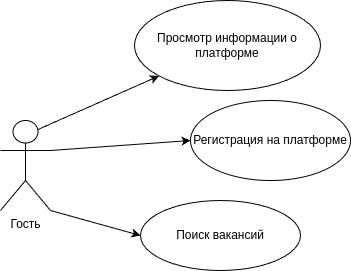
\includegraphics[width=1\linewidth]{p1}
	\caption{Диаграмма прецедентов для категории пользователей - гость}
	\label{p1:image}
\end{figure}

Соискателю должны быть доступны следующие функции:

\begin{enumerate}
	\item Авторизация на платформе.
	\item Создание и редактирование резюме.
	\item Поиск вакансий.
	\item Отклик на вакансию.
\end{enumerate}

Прецеденты для соискателя представлены на рисунке ~\ref{p2:image}.

\begin{figure}[H]
	
\includegraphics[width=1\linewidth]{p2}
	\caption{Диаграмма прецедентов для категории пользователей - соискатель}
	\label{p2:image}
\end{figure}

Работодателю должны быть доступны следующие функции:

\begin{enumerate}
	\item Авторизация на платформе.
	\item Публикация вакансии.
	\item Просмотр резюме соискателей.
	\item Просмотр откликов на вакансию.
\end{enumerate}

\begin{figure}[H]
	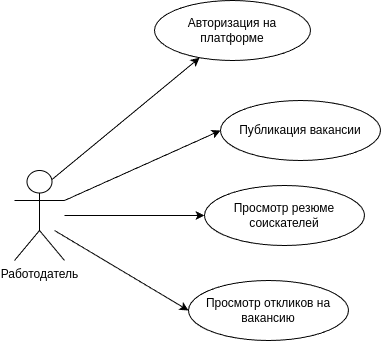
\includegraphics[width=1\linewidth]{p3}
	\caption{Диаграмма прецедентов для категории пользователей - работодатель}
	\label{p3:image}
\end{figure}

Aдминистратору должны быть доступны следующие функции:

\begin{enumerate}
	\item Управление пользователями.
	\item Модерация вакансий и резюме.
	\item Управление информационными разделами.
\end{enumerate}

\begin{figure}[H]
	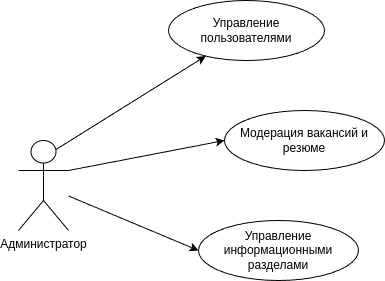
\includegraphics[width=1\linewidth]{p4}
	\caption{Диаграмма прецедентов для категории пользователей - администратор}
	\label{p4:image}
\end{figure}

\subsection{Требования к оформлению документации}

Разработка программной документации и программного изделия должна производиться согласно ГОСТ 19.102-77 и ГОСТ 34.601-90. Единая система программной документации.

\section{Технический проект}
\subsection{Общая характеристика организации решения задачи}

Необходимо спроектировать и разработать web-платформу для поиска работы, которая должна способствовать эффективному взаимодействию между соискателями и работодателями на рынке труда.

Платформа представляет собой набор взаимосвязанных электронных страниц, сгруппированных по разделам, содержащих текстовую, графическую и мультимедийную информацию (например, описания вакансий, резюме, изображения). Платформа размещается в Интернете по уникальному доменному имени, например, www.jobplatform.ru. Каждая страница платформы — это документ, созданный с использованием современных технологий веб-разработки (PHP, CSS, JavaScript и других).

\subsection{Обоснование выбора технологии проектирования}

На сегодняшний день информационный рынок, поставляющий программные решения в выбранной сфере, предлагает множество продуктов, позволяющих достигнуть поставленной цели – разработки web-платформы.

\subsubsection{Описание используемых технологий и языков программирования}

В процессе разработки web-сайта используются программные средства и языки программирования. Каждое программное средство и каждый язык программирования применяется для круга задач, при решении которых они необходимы.

\subsubsection{Фреймворк PHP (Symfony)}

Symfony — это высокопроизводительный фреймворк, основанный на языке программирования PHP, предназначенный для создания серверной части (backend) web-приложений. PHP используется для написания сценариев, которые исполняются на сервере и формируют динамические страницы платформы, такие как списки вакансий, личные кабинеты и результаты поиска. Symfony предоставляет мощные инструменты для работы с базами данных, обработки запросов через REST API и обеспечения безопасности (например, JWT-аутентификация).

\paragraph{Достоинства фреймворка Symfony}

Основные преимущества Symfony включают:

\begin{enumerate}
	\item Модульная структура, упрощающая масштабирование и поддержку кода.
	\item Встроенные механизмы валидации форм и управления пользователями, что идеально для реализации регистрации, авторизации и обработки резюме/вакансий.
	\item Интеграция с ORM (например, Doctrine) для удобной работы с базой данных (MySQL/PostgreSQL).
	\item Высокая производительность и поддержка современных стандартов PHP.
\end{enumerate}


\subsubsection{Язык программирования JavaScript (Vue.js)}

JavaScript — объектно-ориентированный язык программирования, используемый для создания интерактивных интерфейсов на стороне клиента. В рамках проекта применяется фреймворк Vue.js, который расширяет возможности JavaScript для построения динамического и divisions (e.g., Vue.js) фронтенда платформы. Vue.js позволяет создавать отзывчивый и интерактивный интерфейс, включая формы для резюме, фильтры поиска и карточки вакансий, без необходимости перезагрузки страницы.

\paragraph{Достоинства языка JavaScript}

Основные преимущества Vue.js:

\begin{enumerate}
	\item Компонентный подход, упрощающий разработку модульных интерфейсов (например, карточки вакансий, формы отклика).
	\item Реактивное обновление данных, обеспечивающее плавное взаимодействие (например, обновление списка вакансий при изменении фильтров).
	\item Лёгкая интеграция с REST API (Symfony) для получения данных с сервера.
	\item Кросс-браузерная совместимость, минимизирующая проблемы с отображением в разных браузерах.
\end{enumerate}

\subsection{Архитектура программной системы}

Диаграмма компонентов описывает физическую архитектуру web-платформы для поиска работы. Она иллюстрирует структуру системы, определяя зависимости между программными компонентами, включая исходный и исполняемый код.

На рисунке \ref{dc:image} изображена архитектура программной системы.

\begin{figure}[ht]
\center{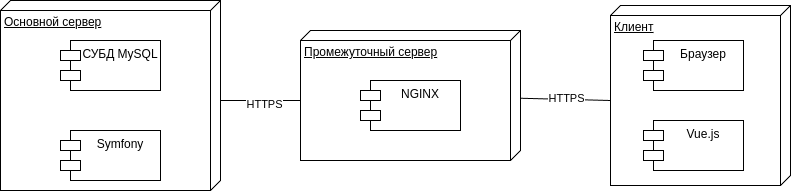
\includegraphics[width=1\linewidth]{dc}}
\caption{Архитектура программной системы}
\label{dc:image}
\end{figure}

Программно-информационная система состоит из следующих компонентов:

\begin{enumerate}
	\item Клиентская часть представлена устройством пользователя (ПК, смартфон или планшет), на котором установлен веб-браузер (например, Chrome, Firefox, Safari). В браузере работает Vue.js Frontend — клиентское приложение, обеспечивающее пользовательский интерфейс платформы. Через интерфейс пользователи (соискатели и работодатели) могут регистрироваться, создавать и редактировать резюме или вакансии, выполнять поиск по вакансиям/резюме и отправлять отклики. Взаимодействие между клиентской частью и сервером осуществляется по защищённому протоколу HTTPS, что гарантирует безопасность передачи данных, таких как личная информация пользователей и их действия на платформе.
	\item Промежуточный сервер реализован с использованием Nginx, который выполняет роль связующего звена между клиентской частью и основным сервером.
	\item Основной сервер реализован с использованием фреймворка Symfony, который отвечает за обработку запросов от клиентской части через REST API. Symfony обеспечивает бизнес-логику платформы, включая:
	\begin{enumerate}
		\item Управление пользователями (регистрация, авторизация, управление профилями).
		\item Обработку данных о вакансиях и резюме (создание, редактирование, публикация).
		\item Поиск и фильтрацию (например, по ключевым словам, локации, зарплате).
		\item Обработку откликов на вакансии.
	\end{enumerate}
	Для хранения данных используется СУБД MySQL (или PostgreSQL), интегрированная с Symfony через ORM Doctrine, что упрощает управление данными и обеспечивает высокую производительность.
\end{enumerate}

\subsection{Структура базы данных}

Сущности и отношение между таблицами базы данных отражены на
рисунке \ref{bd:image}

\begin{figure}[H]
	\center{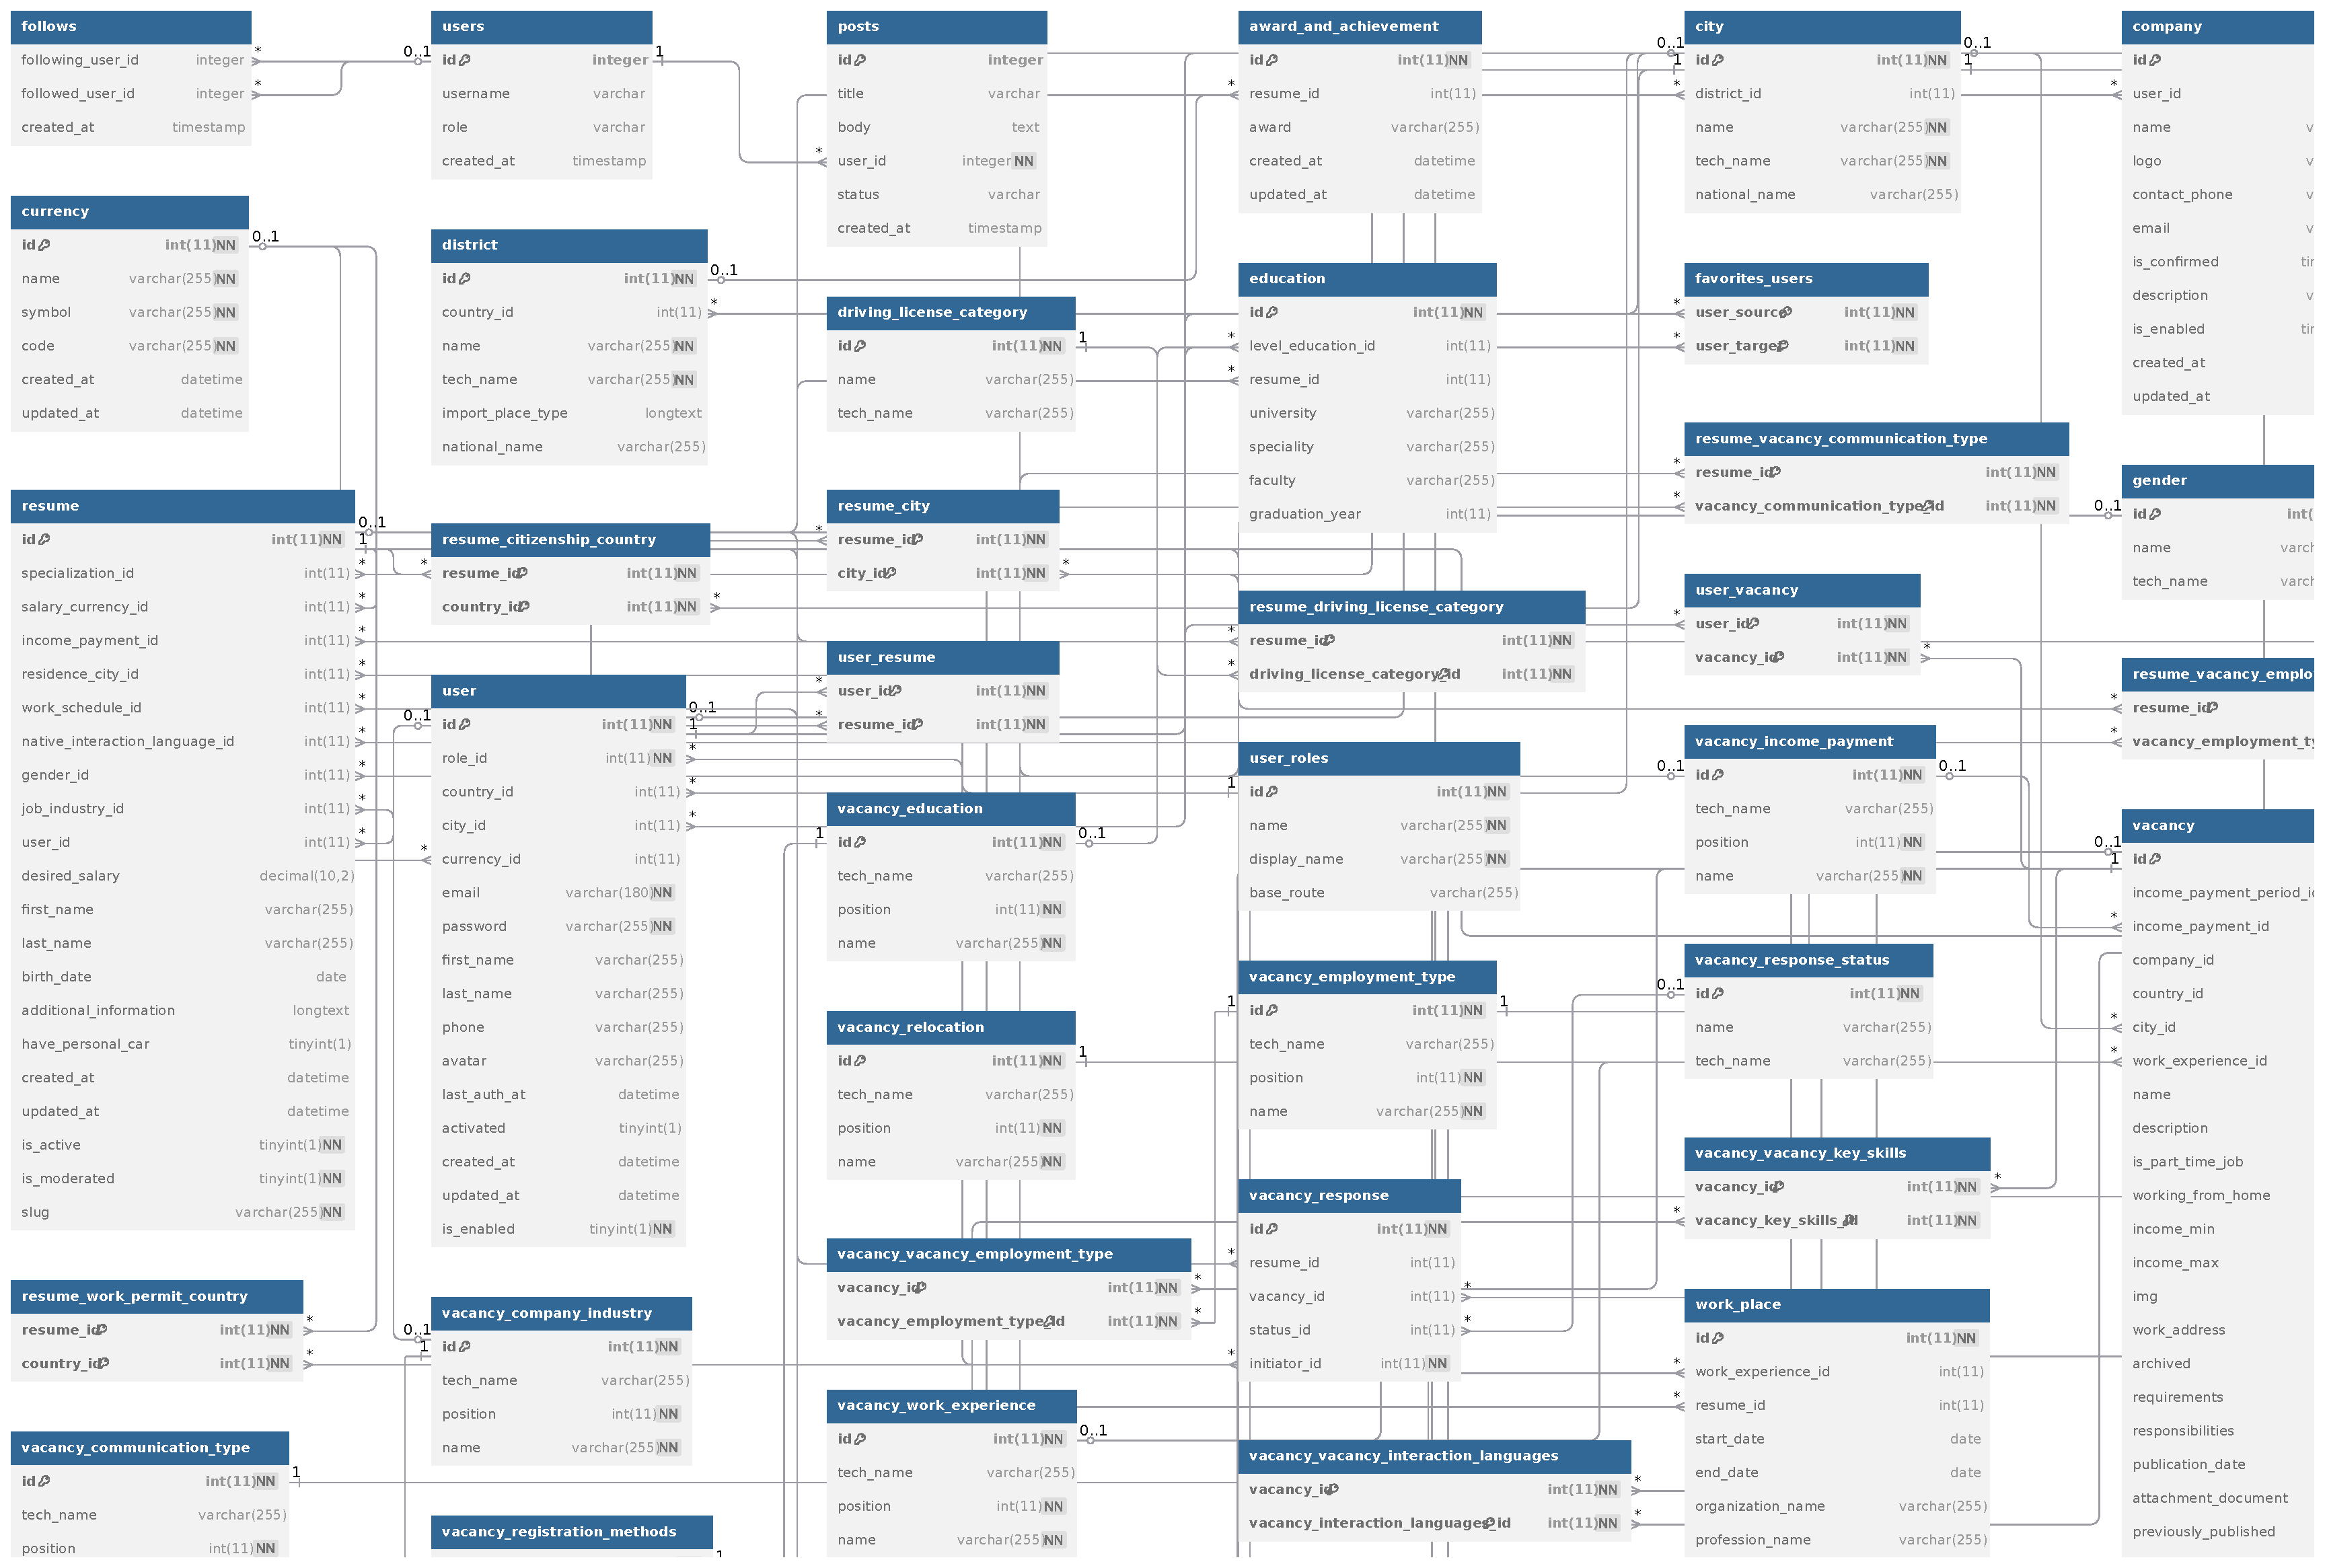
\includegraphics[width=1\linewidth]{bd}}
	\caption{ER-диаграмма}
	\label{bd:image}
\end{figure}


В таблице \ref{ssevsws:table} представлена структура таблицы resume.

\begin{xltabular}{\textwidth}{|l|l|p{1.7cm}|X|}
	\caption{Таблица resume \label{ssevsws:table}}\\ \hline
	\centrow Тип ключа & \centrow Имя столбца & \centrow Тип
	данных & \centrow Обязательность \\ \hline
	\thead{1} & \thead{2} & \centrow 3 & \centrow 4 \\ \hline
	\endfirsthead
	\continuecaption{Продолжение таблицы \ref{ssevsws:table}}
	\thead{1} & \thead{2} & \centrow 3 & \centrow 4 \\ \hline
	\finishhead
	primary key & id & integer & true \\ \hline 
	foreign key & specialization & integer & true \\ \hline 
	 & desiredSalary & string & true \\ \hline 
	 & firstName & string & true \\ \hline 
	 & lastName & string & true \\ \hline 
	 & birthDate & date & true \\ \hline 
	 & workPlace & string & false \\ \hline
	 & education & string & false \\ \hline
	foreign key & employmentType & integer & true \\ \hline
	foreign key & user & integer & true \\ \hline
\end{xltabular}

В таблице \ref{vacancy:table} представлена структура таблицы vacancy.

\begin{xltabular}{\textwidth}{|l|l|p{1.7cm}|X|}
	\caption{Таблица vacancy \label{vacancy:table}}\\ \hline
	\centrow Тип ключа & \centrow Имя столбца & \centrow Тип
	данных & \centrow Обязательность \\ \hline
	\thead{1} & \thead{2} & \centrow 3 & \centrow 4 \\ \hline
	\endfirsthead
	\continuecaption{Продолжение таблицы \ref{vacancy:table}}
	\thead{1} & \thead{2} & \centrow 3 & \centrow 4 \\ \hline
	\finishhead
	primary key & id & integer & true \\ \hline 
	 & name & string & true \\ \hline 
	foreign key & specializations & integer & true \\ \hline 
	& description & string & true \\ \hline 
	& incomeMin & string & true \\ \hline 
	& icomeMax & string & true \\ \hline 
   foreign key & incomePayment & integer & true \\ \hline
	foreign key & company & integer & true \\ \hline
	& requirements & string & false \\ \hline
	& responsibilities & string & false \\ \hline
	foreign key & city & integer & true \\ \hline
	foreign key & country & integer & true \\ \hline
	foreign key & employmentType & integer & true \\ \hline
\end{xltabular}

В таблице \ref{user:table} представлена структура таблицы user.

\begin{xltabular}{\textwidth}{|l|l|p{1.7cm}|X|}
	\caption{Таблица vacancy \label{user:table}}\\ \hline
	\centrow Тип ключа & \centrow Имя столбца & \centrow Тип
	данных & \centrow Обязательность \\ \hline
	\thead{1} & \thead{2} & \centrow 3 & \centrow 4 \\ \hline
	\endfirsthead
	\continuecaption{Продолжение таблицы \ref{user:table}}
	\thead{1} & \thead{2} & \centrow 3 & \centrow 4 \\ \hline
	\finishhead
	primary key & id & integer & true \\ \hline 
	& email & string & true \\ \hline 
	foreign key & roles & integer & true \\ \hline 
	& password & string & true \\ \hline 
	& firstName & string & true \\ \hline 
	& lastName & string & true \\ \hline 
	& phone & string & true \\ \hline
	foreign key & country & integer & false \\ \hline
	foreign key & companies & integer & false \\ \hline
	foreign key & vacancyFavorites & integer & false \\ \hline
	foreign key & resumeFavorites & integer & false \\ \hline
	foreign key & resumes & integer & false \\ \hline
	foreign key & favoriteUsers & integer & false \\ \hline
\end{xltabular}

В таблице \ref{company:table} представлена структура таблицы company.

\begin{xltabular}{\textwidth}{|l|l|p{1.7cm}|X|}
	\caption{Таблица vacancy \label{company:table}}\\ \hline
	\centrow Тип ключа & \centrow Имя столбца & \centrow Тип
	данных & \centrow Обязательность \\ \hline
	\thead{1} & \thead{2} & \centrow 3 & \centrow 4 \\ \hline
	\endfirsthead
	\continuecaption{Продолжение таблицы \ref{company:table}}
	\thead{1} & \thead{2} & \centrow 3 & \centrow 4 \\ \hline
	\finishhead
	primary key & id & integer & true \\ \hline 
	foreign key & user & integer & true \\ \hline 
	& name & string & true \\ \hline 
	& contactPhone & string & false \\ \hline 
	& email & string & false \\ \hline 
	& description & string & false \\ \hline
	foreign key & vacancies & integer & false \\ \hline
\end{xltabular}

В таблице \ref{country:table} представлена структура таблицы company.

\begin{xltabular}{\textwidth}{|l|l|p{1.7cm}|X|}
	\caption{Таблица vacancy \label{country:table}}\\ \hline
	\centrow Тип ключа & \centrow Имя столбца & \centrow Тип
	данных & \centrow Обязательность \\ \hline
	\thead{1} & \thead{2} & \centrow 3 & \centrow 4 \\ \hline
	\endfirsthead
	\continuecaption{Продолжение таблицы \ref{country:table}}
	\thead{1} & \thead{2} & \centrow 3 & \centrow 4 \\ \hline
	\finishhead
	primary key & id & integer & true \\ \hline 
	& name & string & true \\ \hline 
	& techName & string & true \\ \hline 
	foreign key & districts & string & false \\ \hline 
\end{xltabular}

В таблице \ref{district:table} представлена структура таблицы district.

\begin{xltabular}{\textwidth}{|l|l|p{1.7cm}|X|}
	\caption{Таблица vacancy \label{district:table}}\\ \hline
	\centrow Тип ключа & \centrow Имя столбца & \centrow Тип
	данных & \centrow Обязательность \\ \hline
	\thead{1} & \thead{2} & \centrow 3 & \centrow 4 \\ \hline
	\endfirsthead
	\continuecaption{Продолжение таблицы \ref{district:table}}
	\thead{1} & \thead{2} & \centrow 3 & \centrow 4 \\ \hline
	\finishhead
	primary key & id & integer & true \\ \hline 
	& name & string & true \\ \hline 
	& techName & string & true \\ \hline 
	foreign key & country & string & false \\ \hline 
	foreign key & cities & string & false \\ \hline 
\end{xltabular}

В таблице \ref{city:table} представлена структура таблицы city.

\begin{xltabular}{\textwidth}{|l|l|p{1.7cm}|X|}
	\caption{Таблица vacancy \label{city:table}}\\ \hline
	\centrow Тип ключа & \centrow Имя столбца & \centrow Тип
	данных & \centrow Обязательность \\ \hline
	\thead{1} & \thead{2} & \centrow 3 & \centrow 4 \\ \hline
	\endfirsthead
	\continuecaption{Продолжение таблицы \ref{city:table}}
	\thead{1} & \thead{2} & \centrow 3 & \centrow 4 \\ \hline
	\finishhead
	primary key & id & integer & true \\ \hline 
	& name & string & true \\ \hline 
	& techName & string & true \\ \hline 
	foreign key & district & string & false \\ \hline 
\end{xltabular}

\ifПрактика{}\else{
   \section{Рабочий проект}
\subsection{Классы, используемые при разработке сайта}

Можно выделить следующий список классов и их методов, использованных при разработке web-приложения (таблица \ref{class:table}). Пример таблицы с уменьшенным межстрочным интервалом.

\renewcommand{\arraystretch}{0.8} % уменьшение расстояний до сетки таблицы
\begin{xltabular}{\textwidth}{|X|p{2.5cm}|>{\setlength{\baselineskip}{0.7\baselineskip}}p{4.85cm}|>{\setlength{\baselineskip}{0.7\baselineskip}}p{4.85cm}|}
\caption{Описание классов Bitrix, используемых в приложении\label{class:table}}\\
\hline \centrow \setlength{\baselineskip}{0.7\baselineskip} Название класса & \centrow \setlength{\baselineskip}{0.7\baselineskip} Модуль, к которому относится класс & \centrow Описание класса & \centrow Методы \\
\hline \centrow 1 & \centrow 2 & \centrow 3 & \centrow 4\\ \hline
\endfirsthead
\caption*{Продолжение таблицы \ref{class:table}}\\
\hline \centrow 1 & \centrow 2 & \centrow 3 & \centrow 4\\ \hline
\finishhead
CMain & Главный модуль & CMain – главный класс страницы web-приложения. После одного из этапов по загрузке страницы в сценарии становится доступным инициализированный системой объект данного класса с именем \$APPLICATION & void ShowTitle(string property\_code = «title», bool strip\_tags = true)
Выводит заголовок страницы
void SetTitle(string title)
Устанавливает заголовок страницы

void ShowCSS(bool external = true, bool XhtmlStyle = true)
Выводит таблицу стилей CSS страницы\\
\hline CFile & Главный модуль & CFile – Класс для работы с файлами и изображениями & array GetFileArray (int file\_id)
Метод возвращает массив, содержащий описание файла (путь к файлу, имя файла, размер) с идентификатором file\_id
\end{xltabular}
\renewcommand{\arraystretch}{1.0} % восстановление сетки

\subsection{Модульное тестирование разработанного web-сайта}

Модульный тест для класса User из модели данных представлен на рисунке \ref{unitUser:image}.

\begin{figure}[ht]
\begin{lstlisting}[language=Python]
from django.test import TestCase
from .models import *
User = get_user_model()


class ShpoTestCases(TestCase):

    def setUp(self) -> None:
        self.user = User.objects.create(username='testtestovich', password='testtestovich', first_name='Sad', last_name='')

    def test_2(self):

        self.assertEqual(self.user.first_name, 'Sad')
        self.assertEqual(self.user.last_name, 'Cat')
        print((self.user))
        print((self.user.first_name))
        print((self.user.last_name))
\end{lstlisting}  
\caption{Модульный тест класса User}
\label{unitUser:image}
\end{figure}

\subsection{Системное тестирование разработанного web-сайта}

На рисунке \ref{main:image} представлена главная страница сайта «Русатом – Аддитивные технологии».
\newpage % при необходимости можно переносить рисунок на новую страницу
\begin{figure}[H] % H - рисунок обязательно здесь, или переносится, оставляя пустоту
\center{\includegraphics[width=1\linewidth]{main1}}
\center{\includegraphics[width=1\linewidth]{main2}}
\center{\includegraphics[width=1\linewidth]{main3}}
\caption{Главная страница сайта «Русатом – Аддитивные технологии»}
\label{main:image}
\end{figure}

На рисунке \ref{menu:image} представлен динамический вывод заголовков, включающий в себя искомые фразы при поиске фраз.

\begin{figure}[ht]
\center{\includegraphics[width=1\linewidth]{menu}}
\caption{Динамический вывод заголовков}
\label{menu:image}
\end{figure}

На рисунке \ref{enter:image} представлен ввод данных для публикации новости.

\begin{figure}[ht]
\center{\includegraphics[width=1\linewidth]{enter}}
\caption{Ввод данных для публикации очень-очень длинной, интересной и полезной новости}
\label{enter:image}
\end{figure}

   \section*{ЗАКЛЮЧЕНИЕ}
\addcontentsline{toc}{section}{ЗАКЛЮЧЕНИЕ}

Преимущества аддитивных технологий заключается в разнообразии процессов, позволяющих применять их в различных областях производства. Существенным ограничением же является и экономическая составляющая, которая не позволит внедрить аддитивное производство повсеместно.
  
Компании, видя, как развиваются информационные технологии, пытаются использовать их выгодно для своего бизнеса, запуская свой сайт для того, чтобы заявить о своем существовании, проинформировать потенциального клиента об услугах или продуктах, которые предоставляет. 
Для продвижения компании «Русатом – Аддитивные технологии» был разработан веб-сайт на основе системы «1С-Битрикс: Управление сайтом».

Основные результаты работы:

\begin{enumerate}
\item Проведен анализ предметной области. Выявлена необходимость использовать 1С-Битрикс.
\item Разработана концептуальная модель web-сайта. Разработана модель данных системы. Определены требования к системе.
\item Осуществлено проектирование web-сайта. Разработана архитектура серверной части. Разработан пользовательский интерфейс web-сайта.
\item Реализован и протестирован web-сайт. Проведено модульное и системное тестирование.
\end{enumerate}

Все требования, объявленные в техническом задании, были полностью реализованы, все задачи, поставленные в начале разработки проекта, были также решены.

Готовый рабочий проект представлен адаптивной версткой сайта. Сайт находится в публичном доступе, поскольку опубликован в сети Интернет.  

}\fi
\addcontentsline{toc}{section}{СПИСОК ИСПОЛЬЗОВАННЫХ ИСТОЧНИКОВ}

\begin{thebibliography}{9}

    \bibitem{javascript} Ньюхэм, Б. Vue.js в действии / К. Беккет Ньюхэм. – Москва~: Вильямс, 2019. — 360 с. – ISBN 978-5-97060-723-7. – Текст~: непосредственный.
    \bibitem{php} Нобак, М. Год с Symfony: Пишем лучший код с Symfony / М. Нобак. – Санкт-Петербург : Питер, 2015. — 220 с. – ISBN 978-5-496-01432-8. – Текст~: непосредственный.
    \bibitem{start} Потенсье, Ф. Symfony: Быстрый старт / Ф. Потенсье. – Санкт-Петербург : Питер, 2022. — 300 с. – ISBN 978-3-496-52012-4. – Текст~: непосредственный.
    \bibitem{mysql}	Потенсье, Ф. Полное руководство по Symfony / Ф. Потенсье. – Москва~: Вильямс, 2008. — 400 с. – ISBN 978-5-8459-1321-0. – Текст~: непосредственный.
	\bibitem{html5}	Салеки, С. Осваиваем Symfony / С. Салеки. – Москва~: ДМК Пресс, 2017. — 280 с. – ISBN 978-5-97060-512-7. – Текст~: непосредственный.
	\bibitem{htmlcss} Хейди, С. Vue.js 3: Поваренная книга / С. Хейди. – Москва~: Эксмо, 2021. — 420 с. – ISBN 978-5-4461-1678-2. – Текст~: непосредственный.
	\bibitem{htmlcss} Уллман, Л. PHP и MySQL: разработка динамических сайтов / Л. Уллман. – Москва~: Вильямс, 2021. — 720 с. – ISBN 978-5-8459-2003-9. – Текст~: непосредственный.
	\bibitem{htmlcss} Фордун, М. MySQL: справочник разработчика / М. Фордун. – Москва~: ДМК Пресс, 2022. — 600 с. – ISBN 978-5-97060-789-3. – Текст~: непосредственный.
	\bibitem{htmlcss} Фланаган, Д. JavaScript: руководство / Д. Фланаган. – Санкт-Петербург~: Символ-Плюс, 2019. — 1072 с. – ISBN 978-5-93286-315-9. – Текст~: непосредственный.
	\bibitem{htmlcss} Нильсен, Д. PHP 8: руководство разработчика / Д. Нильсен. – Санкт-Петербург~: Питер, 2022. — 480 с. – ISBN 978-5-4461-2034-5. – Текст~: непосредственный.
	\bibitem{htmlcss} Дакетт, Дж. CSS: руководство для начинающих / Дж. Дакетт. – Москва~: Эксмо, 2021. — 448 с. – ISBN 978-5-04-112345-6. – Текст~: непосредственный.
\end{thebibliography}

\ifВКР{\appendix{Представление графического материала}

Графический материал, выполненный на отдельных листах,
изображен на рисунках А.1--А.\arabic{числоПлакатов}.
\setcounter{числоПлакатов}{0}

\renewcommand{\thefigure}{А.\arabic{figure}} % шаблон номера для плакатов

\begin{landscape}

\begin{плакат}
    
\includegraphics[width=0.82\linewidth]{плакат1.png}
    \заголовок{Сведения о ВКРБ}
    \label{pl1:image}      
\end{плакат}

\begin{плакат}
    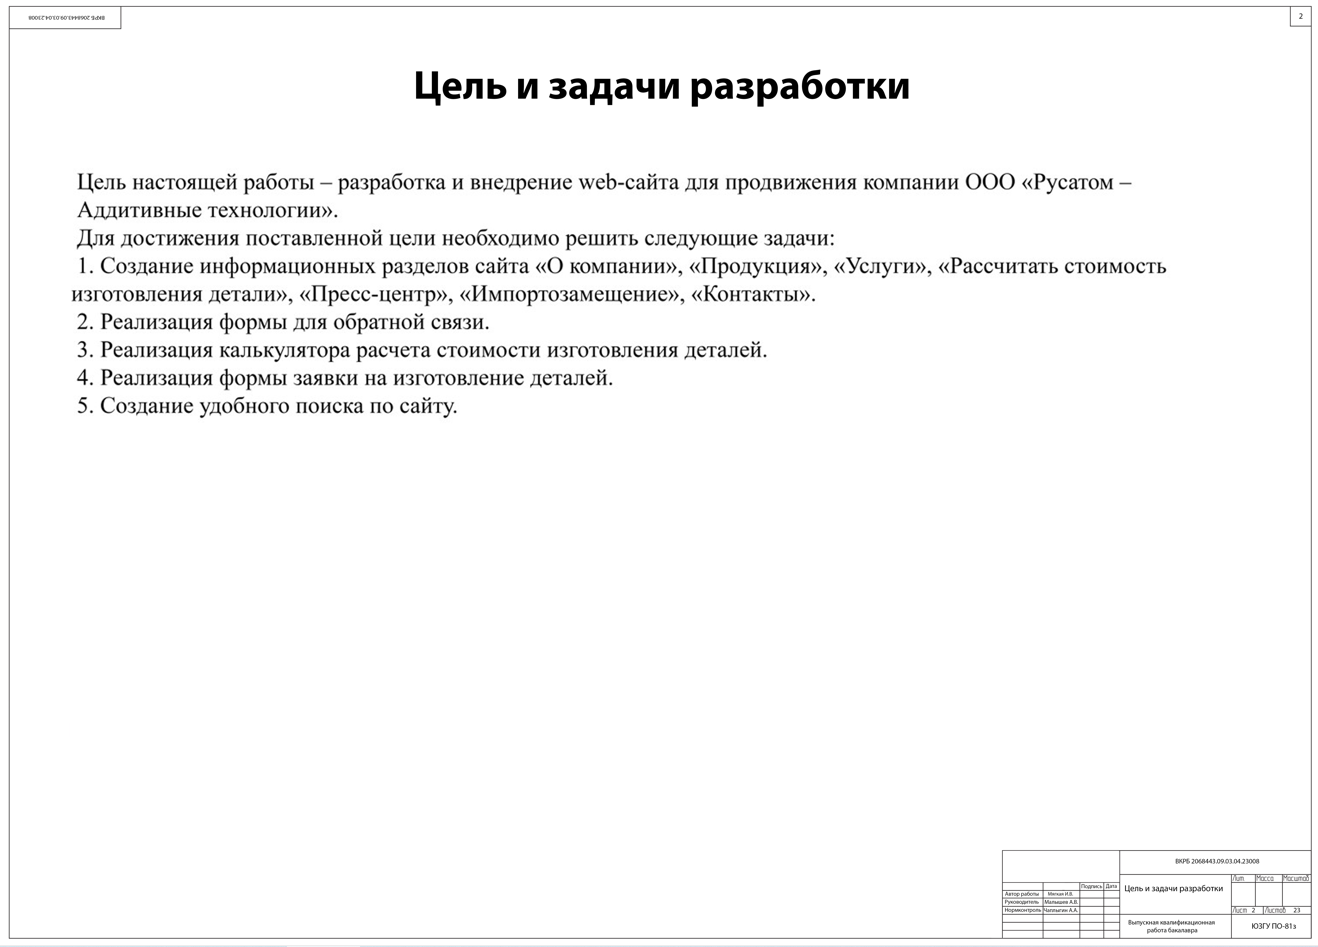
\includegraphics[width=0.82\linewidth]{плакат2.png}
    \заголовок{Цель и задачи разработки}
    \label{pl2:image}      
\end{плакат}

\begin{плакат}
    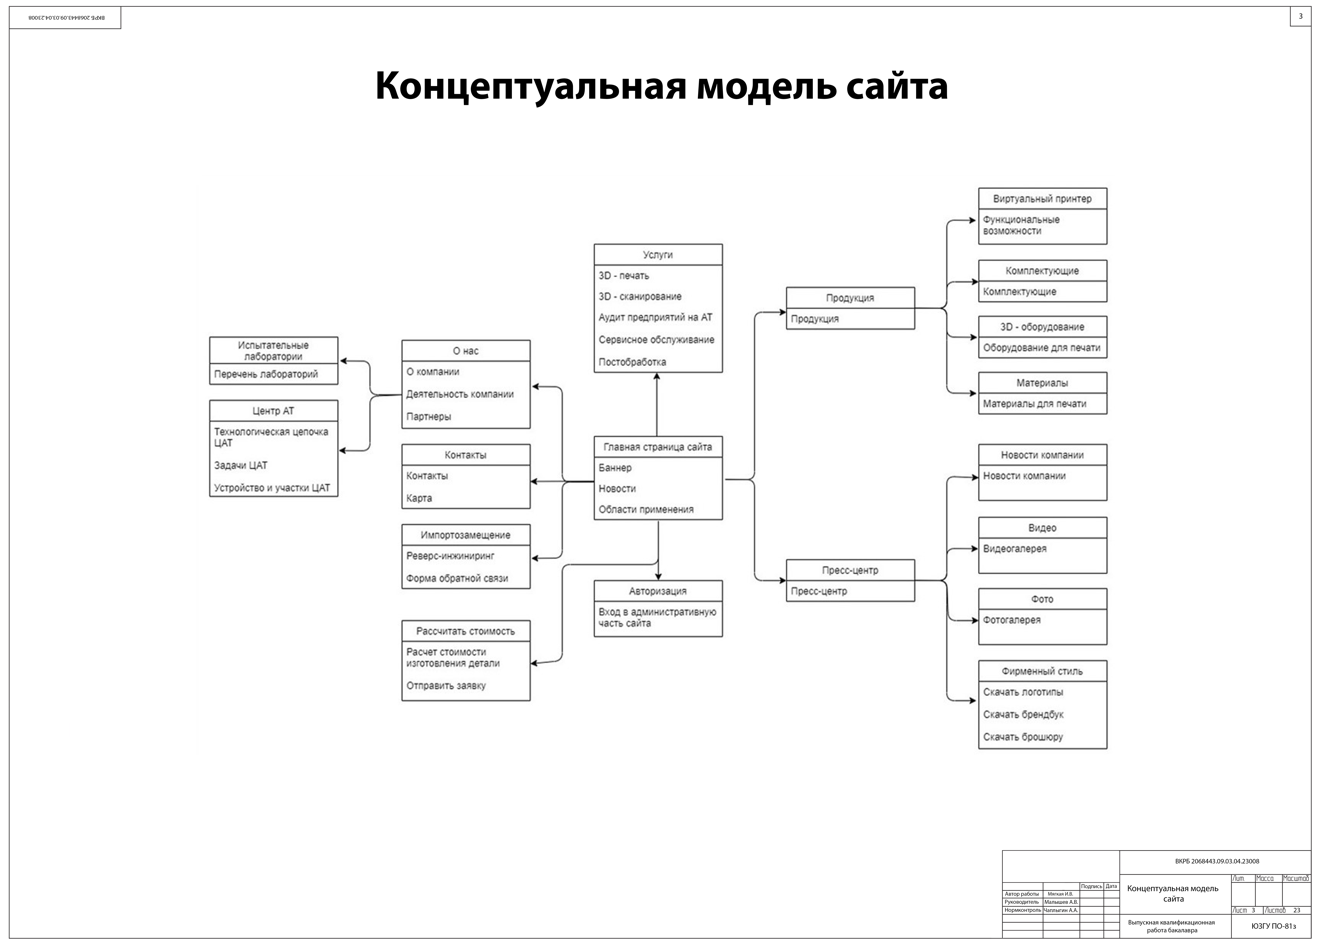
\includegraphics[width=0.82\linewidth]{плакат3.png}
    \заголовок{Концептуальная модель сайта}
    \label{pl3:image}      
\end{плакат}

\begin{плакат}
    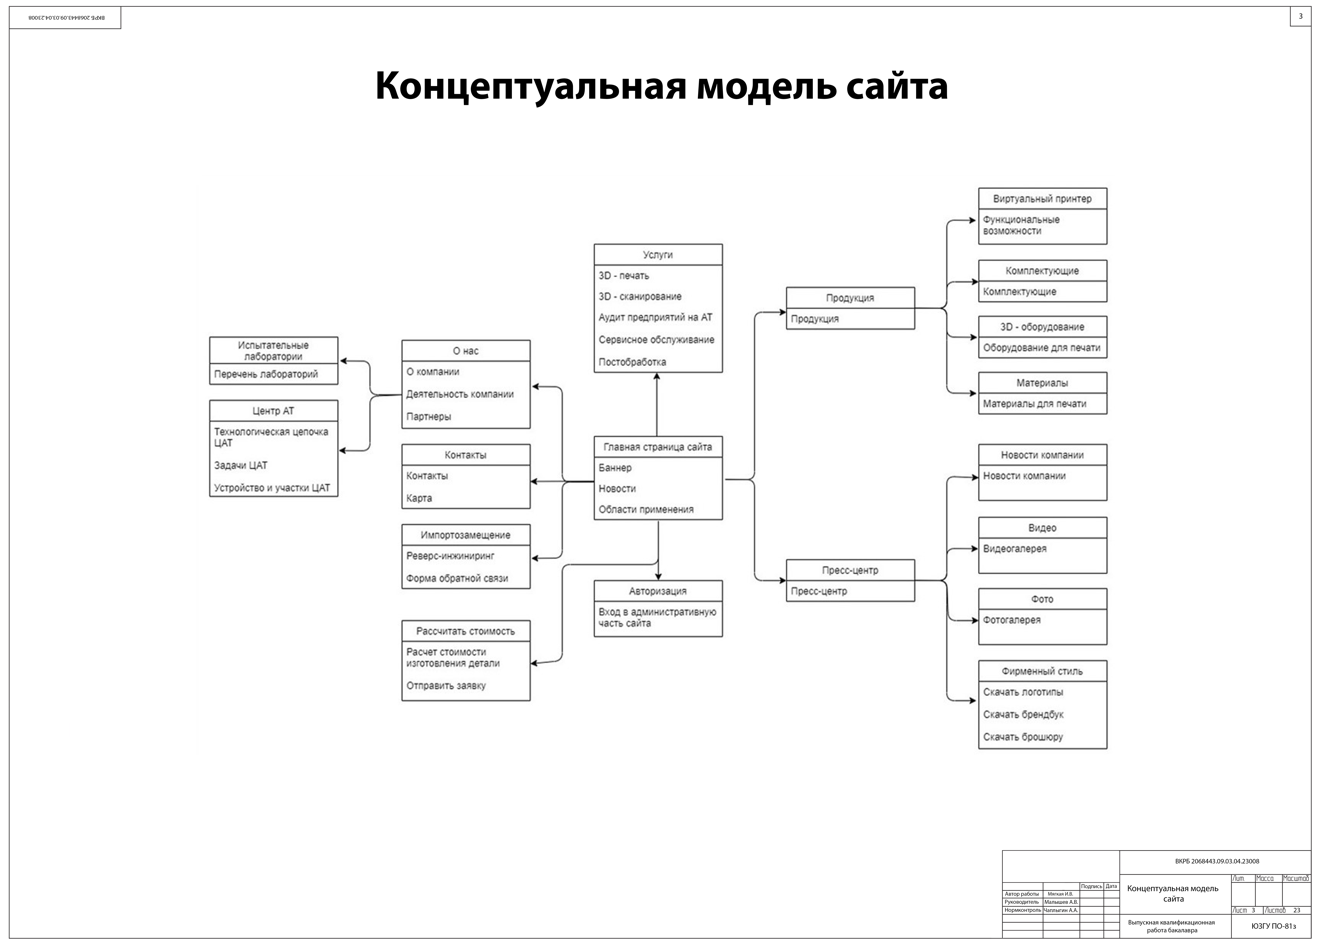
\includegraphics[width=0.82\linewidth]{плакат3.png}
    \заголовок{Еще плакат}
    \label{pl4:image}      
\end{плакат}

\end{landscape}
}\fi
\ifПрактика{}\else{\appendix{Фрагменты исходного кода программы}

main.tex
\lstinputlisting[language=Tex, frame=none]{main.tex}

ТехПроект.tex
\lstinputlisting[language=Tex, frame=none]{ТехПроект.tex}

\ifВКР{
\newpage
\addcontentsline{toc}{section}{На отдельных листах (CD-RW в прикрепленном конверте)}
\noindent
\begin{tabular}{p{5.8cm}C{4.8cm}C{4.8cm}}
   Автор ВКР & \lhrulefill{\fill} & \fillcenter\Автор \\
            \setarstrut{\footnotesize}
           & \footnotesize{(подпись, дата)} & \\
            \restorearstrut
   Руководитель ВКР & \lhrulefill{\fill} & \fillcenter\Руководитель \\
            \setarstrut{\footnotesize}
           & \footnotesize{(подпись, дата)} & \\
            \restorearstrut
   Нормоконтроль & \lhrulefill{\fill} & \fillcenter\Нормоконтроль \\
            \setarstrut{\footnotesize}
           & \footnotesize{(подпись, дата)} & \\
            \restorearstrut
\end{tabular}
\vskip 2cm
\begin{center}
\textbf{Место для диска}
\end{center}
}\fi
}\fi
\end{document}
